\newpage

\section{基本测量}
测量位置, 速度, 亮度等信息.

\subsection{坐标系}

\subsubsection{赤道坐标系}
\begin{figure}[!htb]
    \centering
    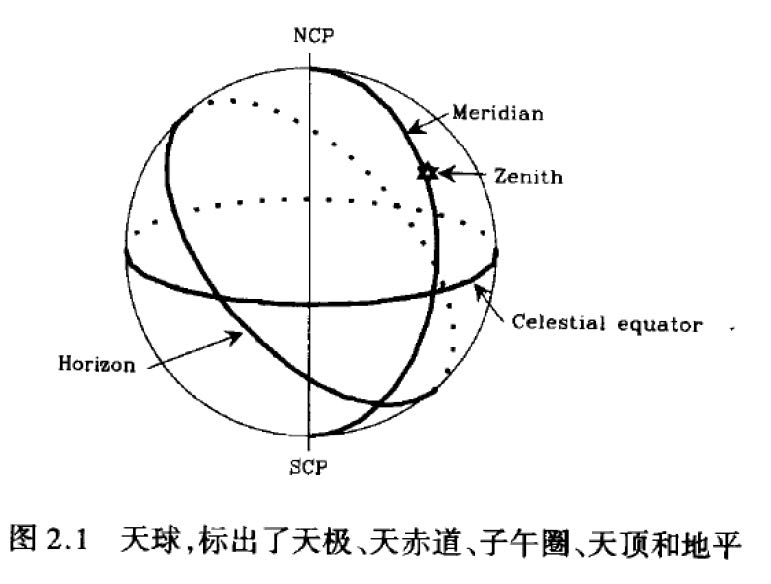
\includegraphics[width=0.42\textwidth]{GA2/赤道坐标系}
    \caption{天球}
\end{figure}
\begin{enumerate}
    \item 天球: 以地球为圆心, 半径无限大的假想球面. 
    \item 北天极 \& 南天极 (NCP \& SCP, North/South Celestial Pole): 地球自转轴与天球的交点. 
    \item 天赤道 (Celestial Equator): 地球赤道面与天球相交平面. 
    \item 对于地面任意观测者, 可以确定一个\hl{天顶} \\(Zenith), \hl{子午圈}(经过 NCP, SCP, Zenith) 和 \hl{地平圈} (可观测的交界处). 由于地球由西向东自传, 天球围绕地面观测者自东向西旋转. 
    \item 天顶距 z: 一个天体与天顶的角距离, 天体的\hl{地平高度}$\alpha=90^{\circ}-z$. 天体穿过子午圈时天顶角距离最小. 
    \item 黄道: 地球围绕太阳转一圈, 太阳在天球上的轨道称为\hl{黄道}. 黄道面与赤道面夹角为 \hl{$23^{\circ}27'$}, 与天赤道的交点分别为\hl{春分点}与\hl{秋分点}. 两次经过春分点的时间间隔称为回归年. 
    \item 赤经: $\alpha$: 为其与春分点之间的角距离, 赤经的0点从春分点开始, 由西向东逐渐增加. 
    \item 赤纬 $\delta$: 从天赤道向北为正, 向南为负, 北天极$\delta=+90^{\circ}$, 南天极$\delta=-90^{\circ}$. 
\end{enumerate}

\subsubsection{银道坐标系}
\begin{figure}[!htb]
    \centering
    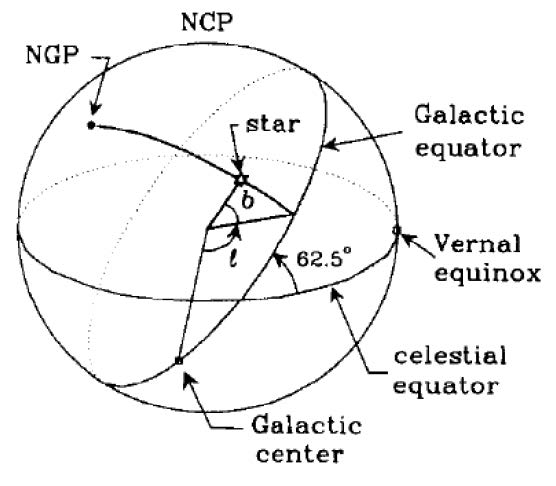
\includegraphics[width=0.309\textwidth]{GA2/银道坐标系}
    \caption{银道坐标系}
\end{figure}

选择银河系的盘在天球上的大圆为银道, 该面与天赤道夹角为$62.87^{\circ}$. 

北银极 (NGP) 为$(\alpha, \delta)=(192.8^{\circ}, 27.12^{\circ}) $. 银心方向为$(\alpha, \delta)=(266.4^{\circ},-28.9^{\circ})$. 

\begin{enumerate}
    \item 银纬 b: 银道面向NGP方向的角度. 
    \item 银经 l: 其距离银心方向的夹角. 
\end{enumerate}

\subsubsection{坐标转换}
可以使用球面夹角公式换算 (具体见ppt )

\subsection{基本概念}

\subsubsection{视差 (parallax)}
\begin{figure}[!htb]
    \centering
    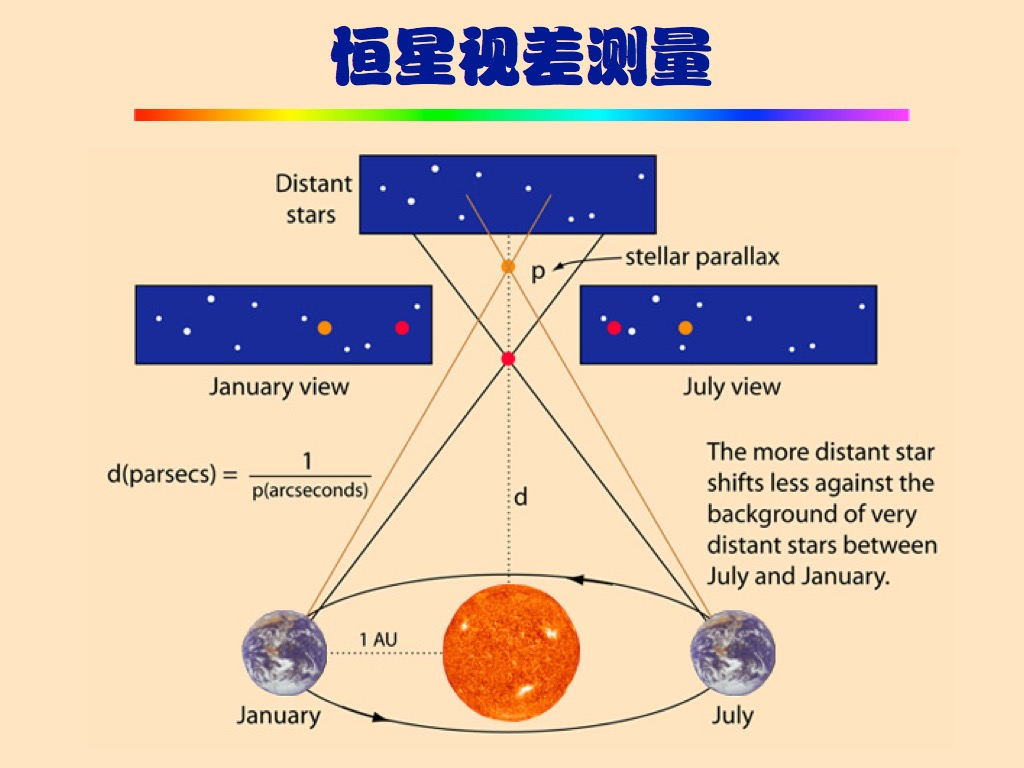
\includegraphics[width=0.47\textwidth]{GA2/视差}
    \caption{视差}
\end{figure}


由于地球公转导致恒星的位置变化. 定义地球的公转平均半径为$r$ (一个天文单位,  $1\mathrm{AU}=1.49\times 10^8$km), 距离为$d$ 的恒星, 其视差为 $w$ (为弧度, 且 $\ll 1$ ), 
\begin{align*}
    \frac{r}{d}=\tan \omega \sim \omega
\end{align*} 

天文距离基本单位为秒差距 (1pc, Parsec), 表示视差为 1 角秒 (arcsec) ($1''=\frac{\pi}{180}\frac{1}{3600}=4.84813\times 10^{-6}$) 的恒星到太阳的距离. 
\begin{align*}
    1\mathrm{pc}=\frac{1\mathrm{AU}}{1''}=206265\mathrm{AU}=3.086\times 10^{13}\mathrm{km}=3.26\text{光年}
\end{align*}

此法一般称为三角视差, 还有测量亮度而得的测光视差(不讲了). 大部分恒星三角视差都是毫角秒量级 (mas, $10^{-3}$arcsec). GAIA卫星的视差测量进度为20uas(微角秒). 

常用天文尺度: Kpc, Mpc, Gpc
\begin{enumerate}
    \item 银河系: 恒星盘直径 $\sim$ 10Kpc, 暗晕半径 200Kpc. 
    \item 星系团的经典尺度: $\sim$ Mpc. 
    \item 星系巡天的经典尺度: $\sim$ Gpc. 
\end{enumerate}

\subsubsection{自行}
\begin{figure}[!htb]
    \centering
    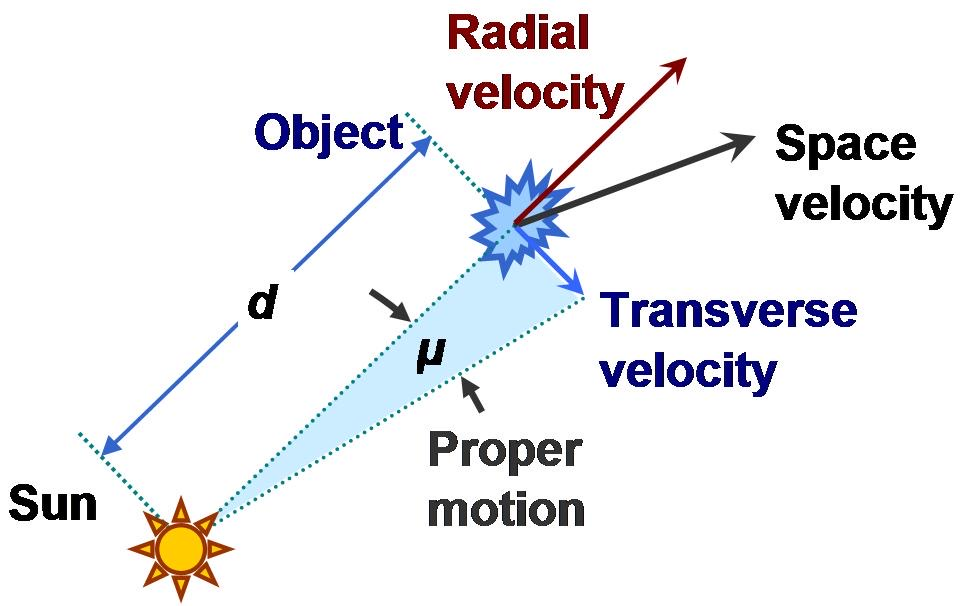
\includegraphics[width=0.42\textwidth]{GA2/自行}
    \caption{自行}
\end{figure}

由于恒星间有相对运动, 在扣除地球公转后, 恒星在与视线垂直方向上的运动分量产生一个角变化率, 称自行. 自行为矢量, $\vec{\mu}$, 以 mas/yr 为单位, 一般方向用位置角 $\theta$ 表示. 自行会改变现有星图排布. 

\subsubsection{视向速度 (Velocity along line-of-sight)}
其测量通过特征光谱的移动, 基本原理是多普勒效应. 后退的光源称为红移, 前进的光源称为蓝移. 

\begin{align*}
    z=\frac{\lambda-\lambda_0}{\lambda_0}=\frac{v\cos\theta}{c}=\frac{v_{los}}{c}=\frac{v_r}{c}
\end{align*}

$z>0$ 红移, $z<0$蓝移. 测量多种元素的特征光谱, 与地球实验室的特征光谱做比较, 可以得知红移. 

\subsubsection{光度与亮度}
光度 (Luminosity, L), 天体在单位时间内辐射总能量为一固有量, 与时间无关. 单位: W or erg/s. 

亮度 (Flux, F)或称流量(F), 观测者单位时间没接收到的天体所辐射的能量, 非内禀量. 单位: W/m${}^2$ or erg/s${}^1$/cm${}^2$. 
\begin{align*}
    L&=F\times S \\
    F&=\frac{L}{4\pi d^2}
\end{align*}

各向同性: 用平分反比定律从距离$d$和流量$F$估计光度. 

恒星光度: $10^{-4}L_{\odot}\sim 10^6 L_{\odot}$.  太阳热光度 (总光度, 所有波长辐射累计): $L_{\odot}=3.86\times 10^{33}erg/s$. 

能量守恒与参考系相关

\subsubsection{光谱 (Spectrum)}
天体在不同波段辐射的能量. 单位: erg/s/nm

光谱特征
\begin{itemize}
    \item 连续谱
    \item 吸收线
    \item 发射线
\end{itemize}

\subsubsection{视星等 (Apparent Magnitude)}
较亮星位1等, 较暗星为6等. 星等与流量之间的换算
\begin{align*}
    m_1-m_2=-2.5\log_{10} \frac{f_1}{f_2}
\end{align*}

\subsubsection{滤光片(Filter)}
截取部分的波长, 给出星等时必须注明滤光片波段. 

不考虑大气吸收, 天体流经滤光片A后的流量为
\begin{align*}
    F=\int_0^{\infty} F_{\lambda}(A) f(\lambda)\, \mathrm{d}\lambda
\end{align*}
$F_{\lambda}(A)$为滤光片A在不同波长处的通光百分比. UBV标准滤光片系统. 滤光片中心位置为有效波长$\lambda_{eff}$, 半高全宽FWHM. VEGA星等系统定义织女星视星等波段为0. 

\subsubsection{颜色color}
测量不同波段星等差可得颜色(色指数), 对于A,B两不同滤光片
\begin{align*}
    m_A-m_B=-2.5\log \frac{\int_0^{\infty} \, \mathrm{d}\lambda F_{\lambda}(A) f(\lambda)}{\int_0^{\infty} \, \mathrm{d}\lambda F_{\lambda}(B) f(\lambda)}
\end{align*}
颜色本质是测量天体在两个不同波段处的流量比, 与距离无关. 测量一个短波与一个长波之间的流量比得到色指数, 如B-V, 提供了恒星的亮度. 

\subsubsection{绝对星等(absolute magnitude)}
一般定义绝对星等为天体处于10pc的视星等. 
\begin{align*}
    \because \, & m=C-2.5\log f\\
    & f=\frac{L}{D^2}
\end{align*}
$f$ 为观测流量, $D$为天体距离, $L$为本征亮度. 

\begin{align*}
    \therefore \,m-M=-2.5\log\frac{f}{F}=5\log \frac{d}{10 \mathrm{pc}}=5\log d - 5 
\end{align*}
$m-M$也叫距离模数, 绝对星等也依赖于测量波段. 

\subsubsection{表面亮度 (surface brightness)}
有时用流量$I$表示, 其与$\mu$有
\begin{align*}
    \mu=C-2.5\log I
\end{align*}

\subsubsection{等亮度线 (isophotal shpae)}
表面亮度相等的区域构成的形状, 可用椭圆来拟合. 

\subsubsection{星系表面亮度分布 (Surface brightness profile)}
亮度分布可用 Sersic Profile 来描述
\begin{align*}
    I(R)=I_0 \exp\left[ -\beta_n\left( \frac{R}{R_e} \right)^{1/n} \right]
\end{align*}
$I_0$为中心表面亮度, $n$为 sersic index. $R_e$为特征半径(半光半径), 其之内包含星系总流量的一半. $\beta_n$为与$n$相关参数, 可近似为$\beta_n=2n=0.324 (n>1)$. 

星系总流量可积分表示为
\begin{align*}
    L=2\pi \int_{0}^{\infty}I(R)R\,\mathrm{d}R=\frac{2\pi n \Gamma (2n)}{\beta_n^{2n}}I_0 R_e^2
\end{align*}

$\Gamma$ 为 gamma function. 

\subsubsection{星系光谱 (spectra)}
光谱(Spectrum)的特征
\begin{itemize}
    \item 连续谱
    \item 吸收线
    \item 发射线
\end{itemize}

星系中发光物质主要恒星, 因此恒星的光谱是构成星系的基础. 恒星的光谱(spectra)分为 O B A F G K M. 恒星辐射接近黑体, 恒星类型与表面大气温度有较好的相关性. 

\quad

\quad

\begin{figure}[htb]
    \centering
    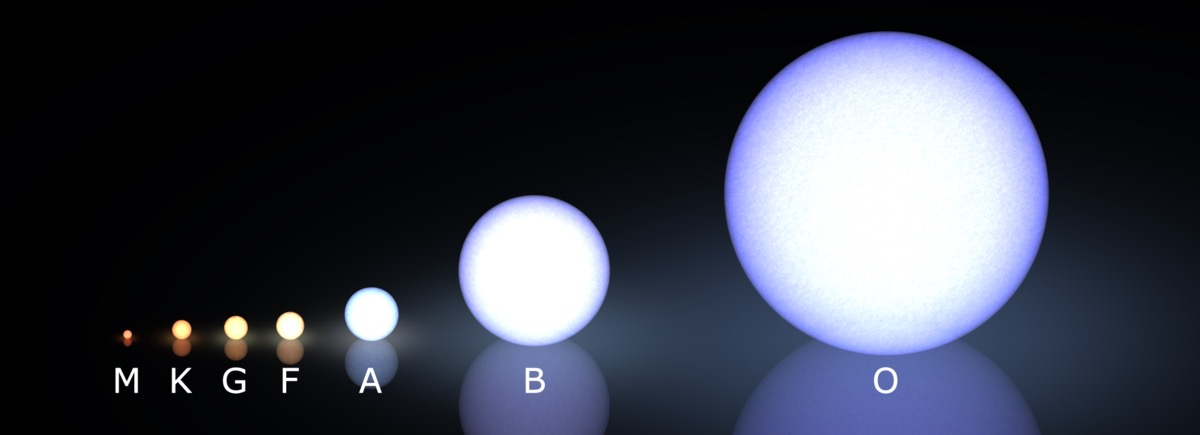
\includegraphics[width=0.42\textwidth]{GA2/恒星光谱}
    \caption{恒星光谱}
\end{figure}

普朗克辐射定律, 在某个波长范围内黑体辐射能量$L(\lambda)\,\mathrm{d}\lambda$: 
\begin{align*}
    L(\lambda)\,\mathrm{d}\lambda =\frac{2hc^2}{\lambda^5}\frac{1}{e^{\frac{hc}{\lambda K T}}-1} \, \mathrm{d}\lambda
\end{align*}
其辐射总能量为$B(T)=\sigma T^4$,$\sigma$为 Stefan-Boltzmann常数. 

不同恒星有不同吸收线. 

\begin{itemize}
    \item 椭圆星系: 基本都是年老恒星, 恒星表面大气产生吸收线(其发射线向各方向辐射), 总体效果为吸收. 无恒星形成区. 
    \item 漩涡星系/星暴星系(starburst): 存在大量恒星形成区(分子云, HII区), 其被年轻恒星高能光子电离, 我们可以看到发射线(HII区背后的分子云导致恒星被完全遮挡). 
\end{itemize} 

\subsubsection{星系介质 (Interstellar medium, ISM)}
主要是气体(99\%)和星际尘埃(1\%). 介质总质量与恒星相当. 

星际介质主要分为: 
\begin{enumerate}
    \item \textbf{中性原子氢气体}: 中性氢广泛存在于恒星际空间, 其分布空间范围比恒星分布延展, 其密度在$[0.1 \sim 10]$ 原子/cm 3, 温度在100-1000K之间.
    
    探测: 星系把部分辐射来自中性H, 其辐射是21cm, 通过红移与蓝移测量速度, 用公式导出速度. 测量中性H可得旋转速度与半径的变化.
    \begin{align*}
        v(r)=\sqrt{\frac{G\cdot(M_{DM}(r)+M_* (r)+M_{gas}(r))}{r}}
    \end{align*}
    \item \textbf{分子云}: 分子云中的主要物质为H2和CO分子, 其主要辐射来自CO的转动跃迁(碰撞激发). 实际观测中H2分子的质量一般从转换因子得到
    \begin{align*}
        X=\frac{N_{H_2}}{I_{CO}}
    \end{align*}
    \item \textbf{电离氢云}: 一般处于恒星形成区, 由于其光谱中含有很强的氢线, 也叫电离氢区(HII). 氢原子被完全电离后发生复合, 产生H${}_{\alpha}$光子等, 同时也会产生气其他元素的发射线, 如OIII. 电离氢区的H${}_{\alpha}$线强度能用来测量星系的恒星形成率. 
    \begin{figure}[!htb]
        \centering
        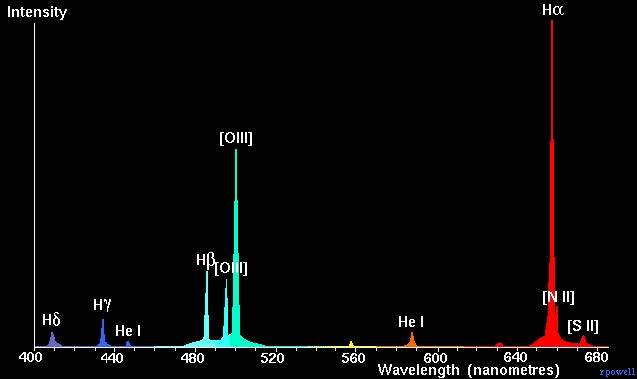
\includegraphics[width=0.479\textwidth]{GA2/电离氢云}
        \caption{非常显著的H${}_{\alpha}$(656.28nm), OIII(496, 500.7 nm), OII (372.7),NII(654.8),发射线}
    \end{figure}
    \item \textbf{星际尘埃 (dust)} 尘埃质量占气体的 1\%, 但是对星系性质有非常强的影响. 
    
    尘埃消光 (dust extinction) 定义为
    \begin{align*}
        A(\lambda)=m_0(\lambda)-m_T(\lambda)
    \end{align*}
    $m_0$为测量值, $m_T$为真值. 
    
    消光依赖于
    \begin{enumerate}
        \item 含量: 数量多, 消光严重. 
        \item 波长: 与组成有关, 短波消光严重, 长波基本不消光. 
    \end{enumerate} 
    短波消光更严重, 导致天体颜色变红, 称为红化. 

    尘埃辐射(dust emission): 尘埃吸收紫外光子, 在红外, 远红外等波段产生辐射在尘埃处于热平衡时, 吸收的总能量等于辐射的总能量. 
\end{enumerate}

\subsection{星系分类}
星系是面源, 有不同形态. 

\subsubsection{哈勃音叉图 (Hubble Tuning Fork)}

分为椭圆, 漩涡, 不规则星系. 椭圆星系也叫早型, 漩涡星系也叫晚型.

\quad

\begin{figure}[!htb]
    \centering
    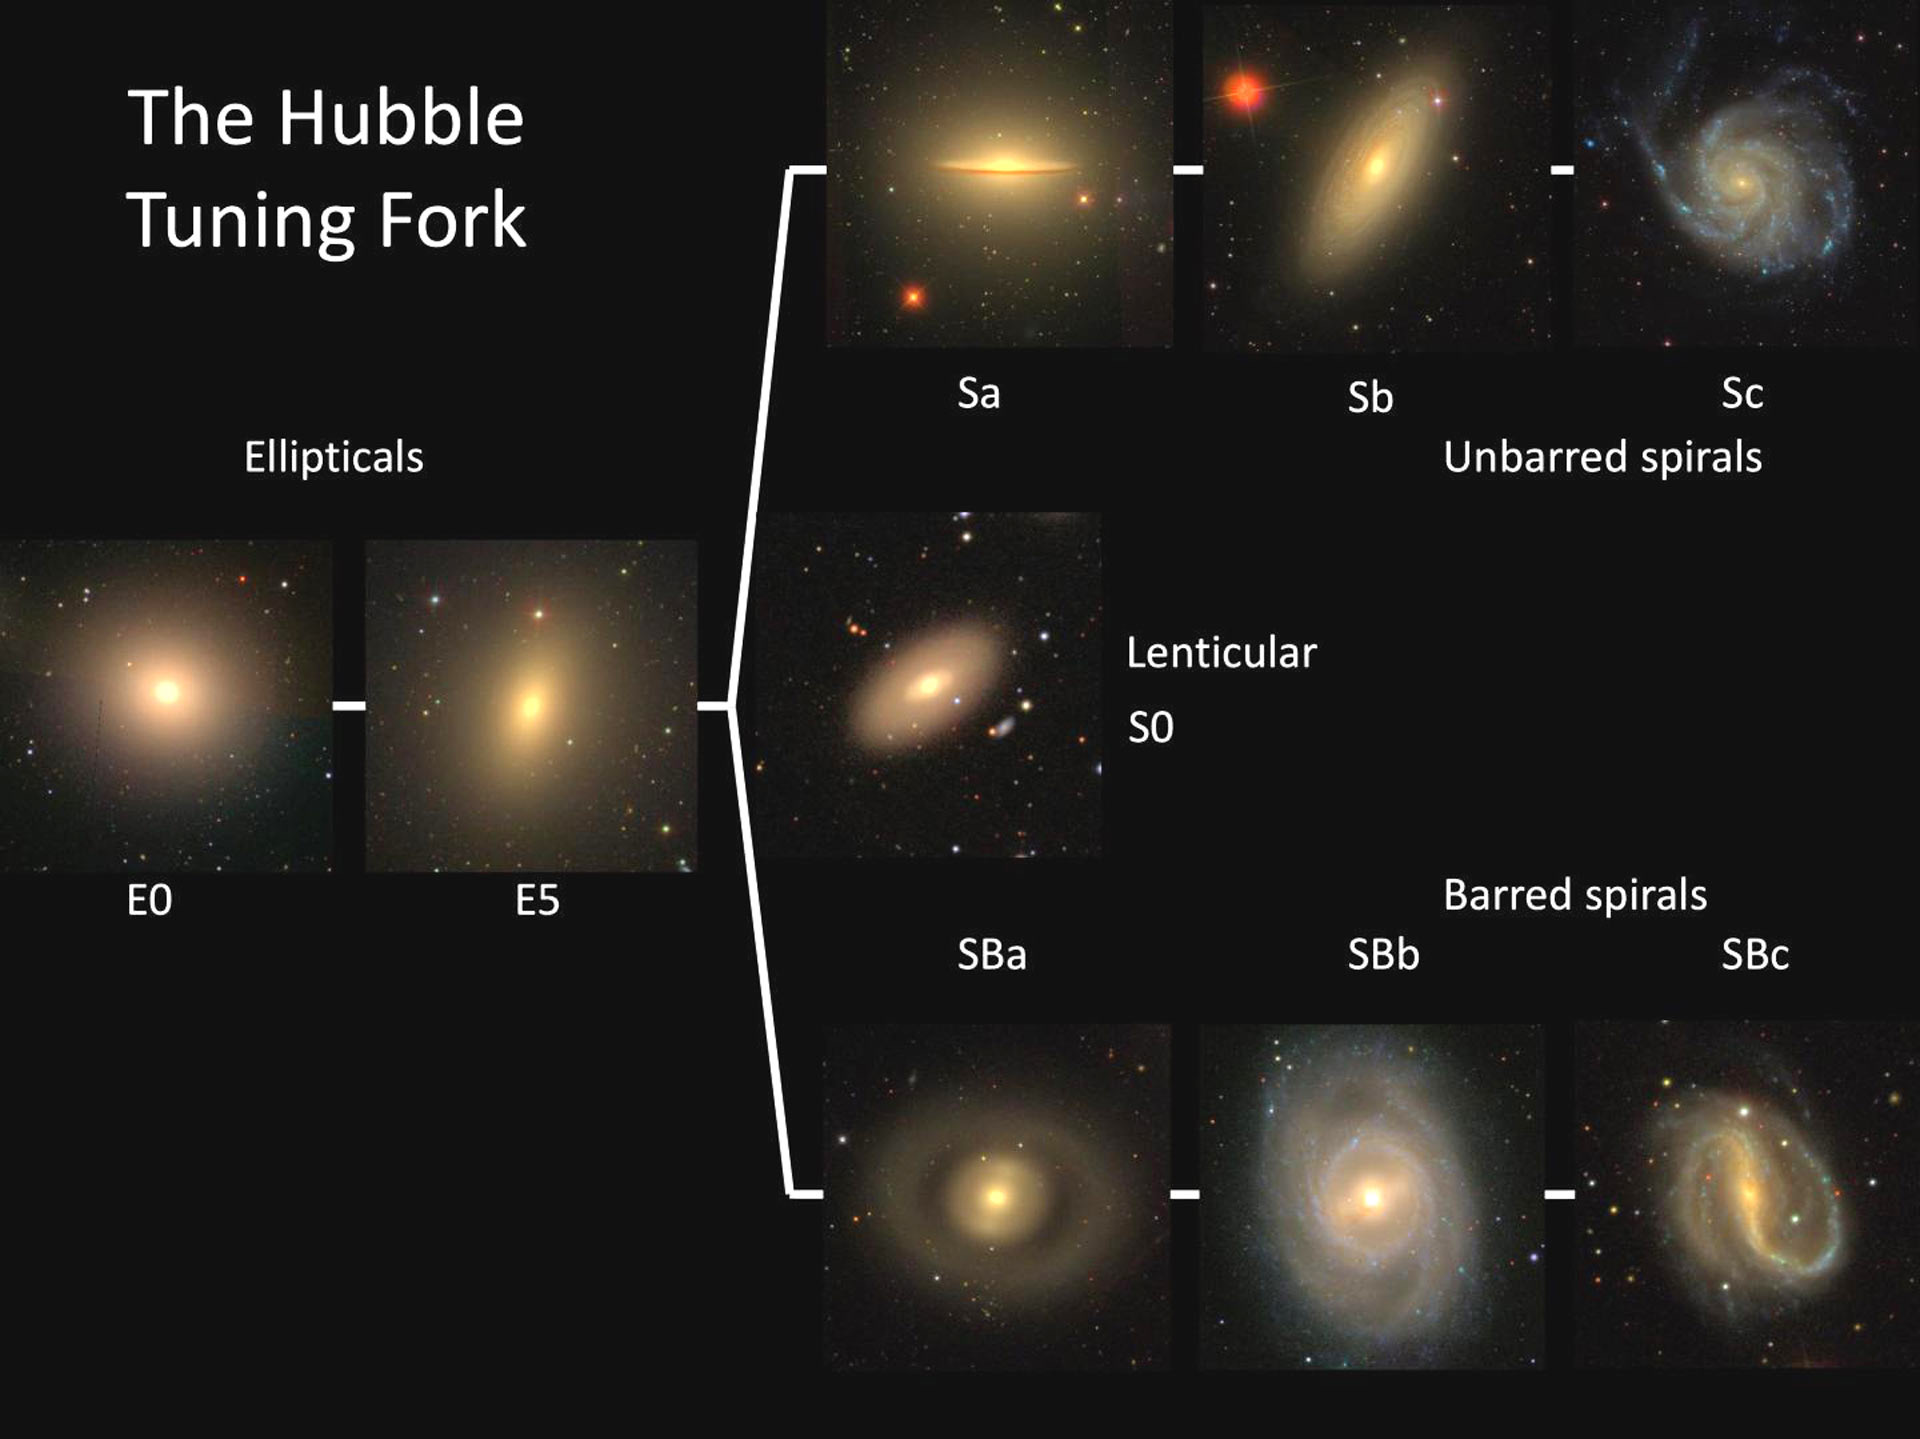
\includegraphics[width=0.309\textwidth]{GA2/哈勃音叉图}
    \caption{哈勃音叉图}
\end{figure} 

\subsubsection{椭圆星系 (Elliptical galaxy)}
符号为$E$, 按椭率大小分为$E_0, E_1, \dots, E_7$ 八个次型, $n=10\frac{a-b}{a}$. 由老年恒星构成, 没有或有少量气体与尘埃. 

\subsubsection{漩涡星系 (Spiral galaxy)}
按核球大小和悬臂的缠绕程度, 分为$S_a, S_b, S_c$三类型. $S_a$ 核球最大, 悬臂最紧. 有大量气体与年轻恒星. 

\subsubsection{棒旋星系 (barred spiral galaxy)}
中间有明显棒的漩涡星系, 根据缠绕程度分为 $SB_{a}$, $SB_b$, $SB_c$. 

\subsection{影响视星等的因素}

\subsubsection{大气吸收} 
由于大气吸收, 滤光片等因素, 实际接受的光子流量为
\begin{align*}
    f=\int_{0}^{\infty} f_v T_v F_v \, \mathrm{d}v
\end{align*}
$T_v$为大气透射, $F_v$为滤光片透射. 

大气吸收与视线上吸收体数量有关, 满足
\begin{align*}
    T \propto  e^{-\alpha}
\end{align*}
$\alpha$成称为光学深度, 与视线方向上空气柱密度成正比. 

$\frac{\alpha}{\alpha_0}$为大气质量, $\alpha_0$为天顶空气柱密度. 对于平面平行大气, 有
\begin{align*}
    \frac{\alpha}{\alpha_0}=\sec z
\end{align*}
$z$是天体的天顶距, 因此大气消光对星等的影响符合
\begin{align*}
    m(z)=k \sec z +C
\end{align*}
$k$为常系数, $m(z)$为恒星在天顶距$z$时的星等. 可通过测量不同处同一天体星等, 可退的天顶大气质量与0大气质量的星等. 

\subsection{巡天测量}

\subsubsection{星系光度函数 (Luminosity function)}
有时也叫质量函数. 指单位体积内某一光度(或质量)范围内的星系数密度. 最重要的观测量之一. 

一般利用Schechter(1976)函数来描述星系的恒星质量(或者光度$L$)函数. 
\begin{align*}
    \phi(L)\ \mathrm{d}L=\phi^*\left(\frac{L}{L^*}\right)^{\alpha}  e^{-L/L^*}\ \mathrm{d} \left(\frac{L}{L^*}\right)
\end{align*}

星系的总密度为
\begin{align*}
    Ng=\int_0^{\infty}\phi(L)\ \mathrm{d}L=\phi^*\Gamma (1+\alpha)
\end{align*}
星系光度密度
\begin{align*}
    \mathcal{L}=\int_0^{\infty}\phi(L)L\ \mathrm{d}L=\phi^* L^* \Gamma (2+\alpha)
\end{align*}
这里$\phi(L)$ 为质量$L, L+\mathrm{d}L$范围内的数密度. 

\begin{figure}[!htb]
    \centering
    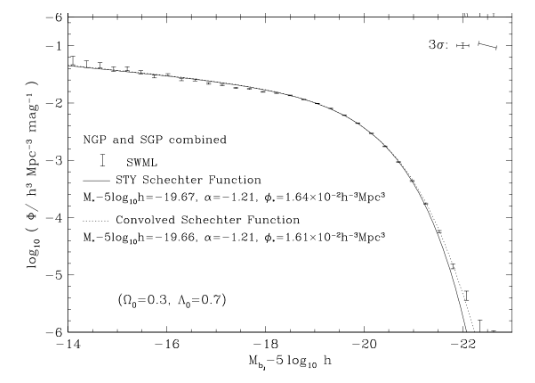
\includegraphics[width=0.479\textwidth]{GA2/星系光度函数}
    \caption{星系光度函数}
\end{figure}

光度函数的几个特征: 
\begin{enumerate}
    \item 超过某个光度星系的数密度:
    \begin{align*}
        n(L)&=\int_L^{\infty} \phi(L)\ \mathrm{d}L\\
        &=\phi^* \int_{L/L^*}^{\infty} \left(\frac{L}{L^*}\right)^{\alpha}  e^{-L/L^*}\ \mathrm{d} \left(\frac{L}{L^*}\right)\\
        &=\phi^*\Gamma\left( \alpha+1,\ \frac{L}{L^*}\right)
    \end{align*}
    当$\frac{L}{L^*}$时, 对于$\alpha<-1$, 星系数密度发散. 
    \item 超过某个光度星系的总光度: 
    \begin{align*}
        T(L)=&=\int_L^{\infty} L\phi(L)\ \mathrm{d}L\\
        &=\phi^* L^* \int_{L/L^*}^{\infty} \left(\frac{L}{L^*}\right)^{\alpha+1}  e^{-L/L^*}\ \mathrm{d} \left(\frac{L}{L^*}\right)\\
        &=\phi^* L^* \Gamma\left( \alpha+2,\ \frac{L}{L^*}\right)
    \end{align*}
\end{enumerate}
\begin{itemize}
    \item $\alpha\le -1$, 星系数密度发散(无穷大)
    \item $\alpha \le -2$, 星系总光度发散. 
    \item 观测表明$-2<\alpha<-1$. 因此并没有光度灾难. 
    
    总光度对于$2+\alpha>0$收敛. 因此暗星系的总数目可以发散(非常大), 但是星系的总光度可以收敛(避免了光度灾难). 
\end{itemize}

\subsubsection{巡天的主要科学发现}
\begin{enumerate}
    \item 颜色或者恒星形成率分布
    \item 星系性质的Scaling relations
    \item 星系中央黑洞质量-核球质量关系: 黑洞质量大约为核球质量的0.1\%. 
    \item 暗物质-恒星质量关系
\end{enumerate}